\documentclass[../main.tex]{subfiles}
\begin{document}
\chapter{Forbruger} \label{Chap:Forbruger}
Forbrugeren er en pulserende belastning, der praktisk talt består af en effekt potentiometer. Der skal implementeres en boost konverter efter energilagret så der kan outputtes en højere og stabil ønsket spænding end hvad energilageret selv kan generere. Ifølge kravspecifikationen skulle der leveres 10 volt til en load. Kontrolleren er den samme som i buck konverteren fra kraftværk sektionen, bare med et par linjer lavet om. 

\section{Boost Konverter}
Der skal implementeres en boost konverter, ved udgangen af energilagringen. Da energilagret har en spænding på ca 5 volt, skal vi have boostet det op til den ønskede 10 volt load. En boost konverter virker lidt på samme måde som en buck konverter, nemlig ved hjælp af at bestemme en duty cycle som giver den rigtige output spænding

\section{Test}
Følgende kravspecifikationer tilhører denne del af projektet
\begin{enumerate}
  \item Spændingen V2 skal være indenfor +/- 1.0 volt
  \item Spændingskilde V2 skal kunne levere min. 150 mA.
  \item Spændingen V2 skal være indenfor +/- 1.0 volt ved en belastningsændring fra 50 mA til 150 mA indenfor 1.0 s.
\end{enumerate}

For at teste Krav 4, belaster vi udgangen af boost konverteren med en tilfældig load og målte spændingen over den. Det kan ses på Figur \ref{fig: Krav 4 Opfyldt} at spændingen (grøn) er 9.91V, og kravet dermed er overholdt.
\begin{figure}[H]
      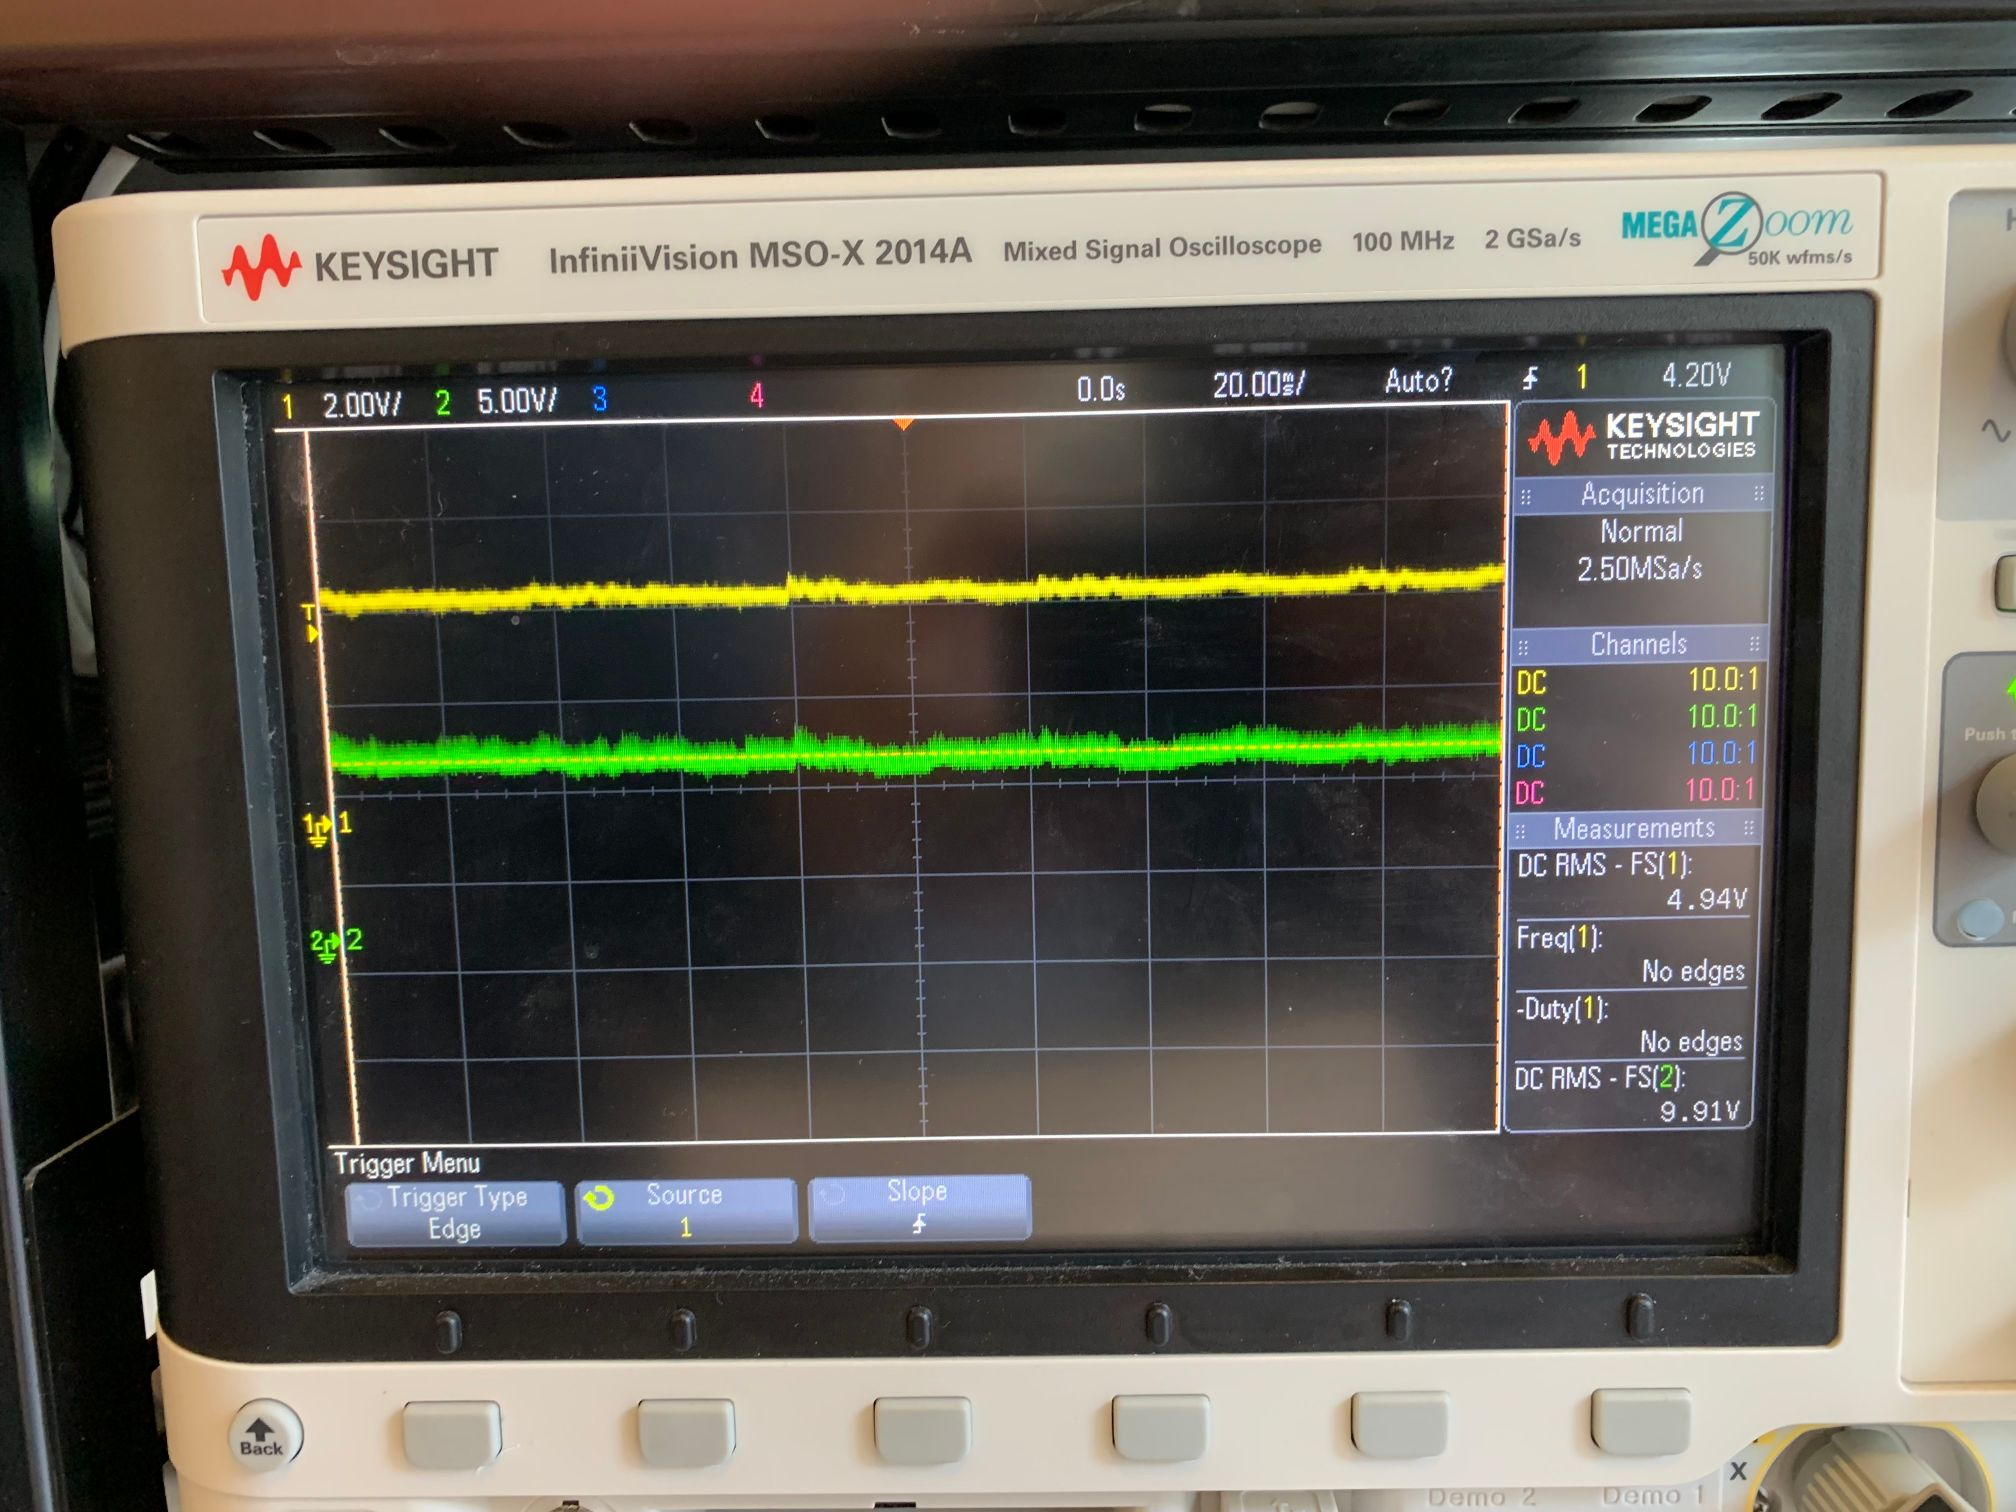
\includegraphics[width=\textwidth]{Dokumentation/Pictures/Krav4.jpg}
     \caption{Krav 4 Opfyldt}
     \label{fig: Krav 4 Opfyldt}
     \end{figure}

For at teste Krav 5, belaster vi udgangen af boost konverteren med 66$\Omega$ hvilket svarer til nogenlunde 150mA. Det kan ses på Figur \ref{fig: Krav 5 og 6 Opfyldt} at spændingen er 9.9V, og kravet dermed er overholdt.

For at teste Krav 6, belaster vi udgangen af boost konverteren med 200$\Omega$ og skifter den derefter hurtigt til 66$\Omega$ hvilket svarer til nogenlunde at hoppe fra 50mA til 150mA. Det kan ses på Figur \ref{fig: Krav 5 og 6 Opfyldt} at spændingen er tilbage på 10V efter 1 sekund (en grid-kasse), og kravet dermed er overholdt.

\begin{figure}[H]
      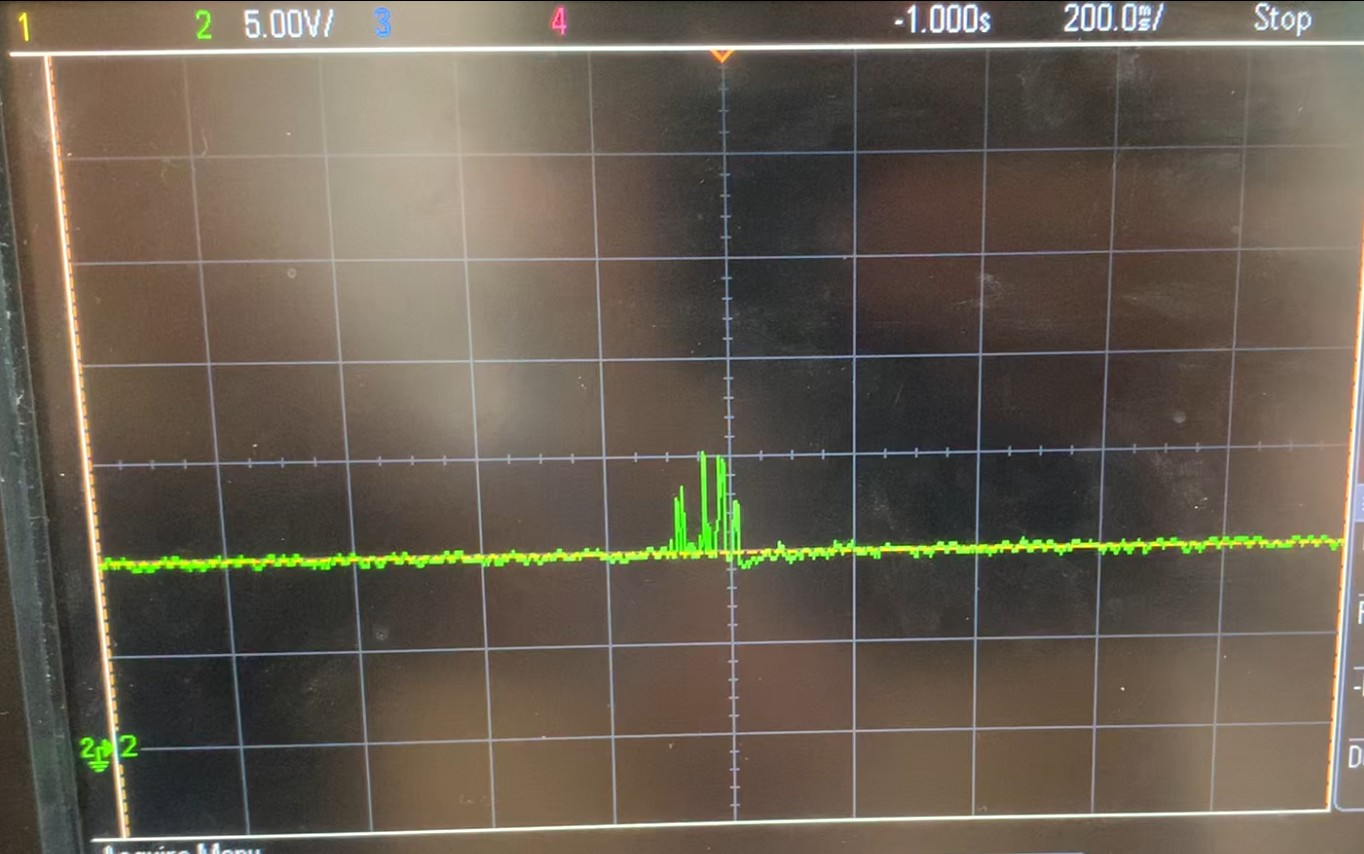
\includegraphics[width=\textwidth]{Dokumentation/Pictures/Krav5og6.jpg}
     \caption{Krav 5 og 6 Opfyldt}
     \label{fig: Krav 5 og 6 Opfyldt}
     \end{figure}

De tre krav er allesammen overholdt, og testen er dermed en succes. 

\end{document}